\documentclass[11pt,english]{article}
\usepackage[a4paper,bindingoffset=0.1in,%
            left=0.5in,right=0.5in,top=0.5in,bottom=0.5in,%
            footskip=.25in]{geometry}
\usepackage[utf8]{inputenc}
\usepackage{graphicx}
\begin{document}
\title{Speech Command Model}
\author{Pradeep Moturi (es16btech11016)}
\date{May 2020}

\sloppy
\maketitle
\setlength{\columnsep}{0.5in}
\twocolumn
\tableofcontents

\section{Introduction}
This is the report of my work done under Dr. G V V Sharma on building a speech command recognition model. 
The model built by me is based on concepts of Convolution, LSTM and Attention.
\section{Create Data}
\begin{enumerate}
    \item Set 16KHz as sampling rate
    \item Record 80 utterances of each command.
    \item Trim each utterance to one second.
    \item Save samples of each command in different folders\\
        Dataset/forward\\
        Dataset/back\\
        Dataset/left\\
        Dataset/right\\
        Dataset/stop
\end{enumerate}
Used Audacity to do this.

\section{Loading Data}
I've used soundfile package to read the .wav. You may choose to use any other package like wavefile, librosa etc to do the same job.\\
As this is one of the slowest part, I've stored the loaded data as a numpy file for ease and speed of access. Now, I can load the data from npy file if repeating the experiment.

\section{Split dataset}
Do a stratified split of the dataset into train and test set with 20\% as test samples.\\
Set a random seed for reproducing the split.

\section{Augment data}
Augment each audio sample by time shifting in 25000 length vectors filled with zeros. \\
Take steps of 500 to create 18 files per sample

\section{Feature Extraction}
MFCCs are most prominent features used in audio processing.
Normalizing the MFCCs over the frequency axis is found to reduce effect of noise.\\
Kapre is a python package that provides layers for audio processing that are compatible with keras and utilize GPU for faster processing. Kapre provides us with a layer basically\\

\textit{Melspectrogram (padding='same', sr=16000, n\_mels=39, n\_dft = 1024, power\_melgram=2.0, return\_decibel\_melgram=True, trainable\_fb=False, trainable\_kernel=False,  name='mel\_stft')}\\

\textbf{Arguments to the layer}\\
\textbf{padding:} Padding when convoluting\\
\textbf{sr:} Sampling rate of audio provided\\
\textbf{n\_mels:} number of coefficients to return\\
\textbf{n\_dft:} width \\
\textbf{power\_melgram:} exponent to raise log-mel-amplitudes before taking DCT. Using power 2 is shown to increase performance by reducing effect of noise\\
\textbf{return\_decibel\_melgram:} If to return log over values\\
\textbf{trainable\_fb:} If filter bank trainable\\
\textbf{trainable\_kernel:} If the kernel is trainable

\section{Building Model}
\subsection{Layers}
\begin{enumerate}
    \item Using Convolutional layers ahead of LSTM is shown to improve performance in several research papers.
    \item BatchNormalization layers are added to improve convergence rate.
    \item Using Bidirectional LSTM is optimal when complete input is available. But this increases the runtime two-fold.
    \item Final output sequence of LSTM layer is used to calculate importance of units in LSTM using a FC layer.
    \item Then take the dot product of unit importance and output sequences of LSTM to get Attention scores of each time step.
    \item Take the dot product of Attention scores and the output sequences of LSTM to get attention vector.
    \item Add an additional FC Layer and then to output Layer with SoftMax Activation.
\end{enumerate}

\subsection{Hyperparameters}
\begin{itemize}
    \item \textbf{sparse\_categorical\_crossentropy} is used as \textbf{Loss} because only output which should be 1 is given instead of One Hot Encoding.
    \item \textbf{sparse\_categorical\_accuracy} is used as performance \textbf{Metric} for the above reason.
    \item \textbf{Adam} is used as \textbf{Optimizer}. Adam is adaptive learning rate optimization algorithm. This is shown to achieve a faster convergence because of having all the features of other optimization algorithms.
\end{itemize}

\section{Training}
\begin{itemize}
    \item Batch size around 15 is found optimal.
    \item Often convergence is achieved in less than 5 epochs.
\end{itemize}

\section{Testing}
\begin{enumerate}
    \item Augment the test set same as training set.
    \item Extract MFCCs using same method as training set
    \item Test set is passed as validation set to fit method of model.
    \item The performance of model on test set is calculated after every epoch.
\end{enumerate}

\section{Visualize Attention}
\begin{enumerate}
    \item Now build a sub model from the trained model. Take same input layer but add ‘AttentionSoftmax’ layer as additional output layer.
    \item Pass MFCCs of test samples to predict method.
    \item Now plot log of Attention Scores and corresponding input vector before taking MFCCs on different axes.
    \item We observe that Attention Scores are high on informative part.
    \begin{figure}[!ht]
    \centering
    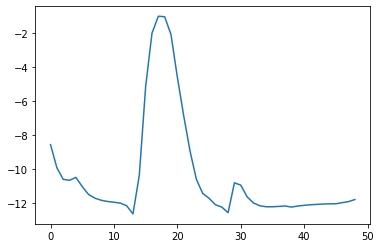
\includegraphics[width=\columnwidth]{./Figs/Attention.png}
    \caption{ Attention Scores}.
    \label{fig: Attention}	
    \end{figure}
    \begin{figure}[!ht]
    \centering
    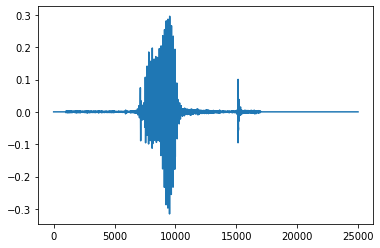
\includegraphics[width=\columnwidth]{./Figs/Sample.png}
    \caption{ Raw sample}.
    \label{fig: Sample}	
    \end{figure}
    
\end{enumerate}

 
\section{Observations}
\begin{itemize}
    \item Smaller batch size is prefferable
    \item Setting power\_melgram=2 of Melspectogram gave faster convergence.
\end{itemize}
\section{Files}
\begin{itemize}
    \item Src/DataGenerator.py: Augments the data
    \item Src/FeatureExtractor.py: Extracts MFCC coefficients
    \item Src/TrainModel.py: Trains model and saves it in h5 file
    \item ColabNotebook.ipynb: Use this for experimental purpose
\end{itemize}

\section{Further}
\begin{itemize}
    \item Different augmentation techniques like adding noise, changing pitch, speed etc.
[https://medium.com/@makcedward/data-augmentation-for-audio-76912b01fdf6]
    \item We can change the arguments to Melspectrogram 
    \item Changing the model architecture like layers and units in layers.
    \item Further the scope of project to check performance on Google’s Speech Command Datasets (v1 and v2) and participate in Kaggle challenge by google
[https://www.kaggle.com/c/tensorflow-speech-recognition-challenge/]

\end{itemize}
%%
\begin{figure}[!ht]
\centering
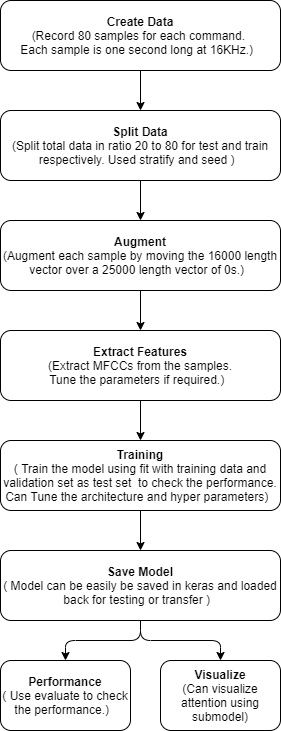
\includegraphics[width=\columnwidth]{./Figs/Flow.png}
\caption{ Data Flow Diagram}.
\label{fig: Flow}	
\end{figure}
%
\begin{figure}[!ht]
\centering
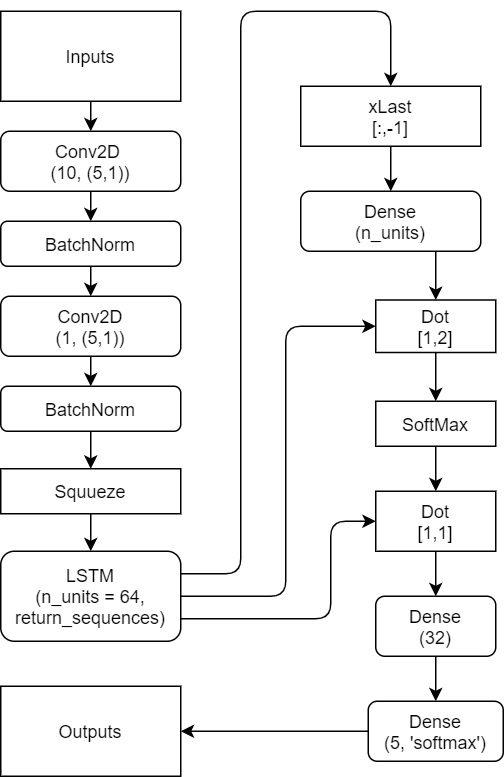
\includegraphics[width=\columnwidth]{./Figs/Model.png}
\caption{ Model Diagram}.
\label{fig: Model}	
\end{figure}


\end{document}